\chapter{Converge-cluster}
Til Converge-cluster er der testet de individuelle services, da det er det eneste kode urørt af framework kode, og er det kode med størst risici for at fejle. Der er flere hundrede tests for converge-cluster spredt ud over alle de anvendte services. Grunden til at frameworket brugt til de forskellige services ikke er testet, er fordi de bliver testet af integrationstests. Hvilket vi har afgjort til at være godt nok til dette projekt. 

Derudover er testene her blevet udviklet løbende og dette betyder at der ikke har været en solid test suite gennem hele forløbet. Det endte ud med at der blev udviklet langt over 100 test cases til Converge-cluster, som gav en solid test suite og at nå gruppens mål på de 100 procent coverage. 
Nedenfor ses de services der er blevet udviklet test cases til:

\begin{itemize}
    \item User-service 
	\item Authenticate-service 
	\item Profile-service 
    \item Bidding-service 
	\item Project-service 
    \item Chat- Service 
	\item Collaboration-service 
	\item collaboration-broker
	\item file-service
	\item Audit-service 
\end{itemize}


\begin{figure}[ht]
    \centering
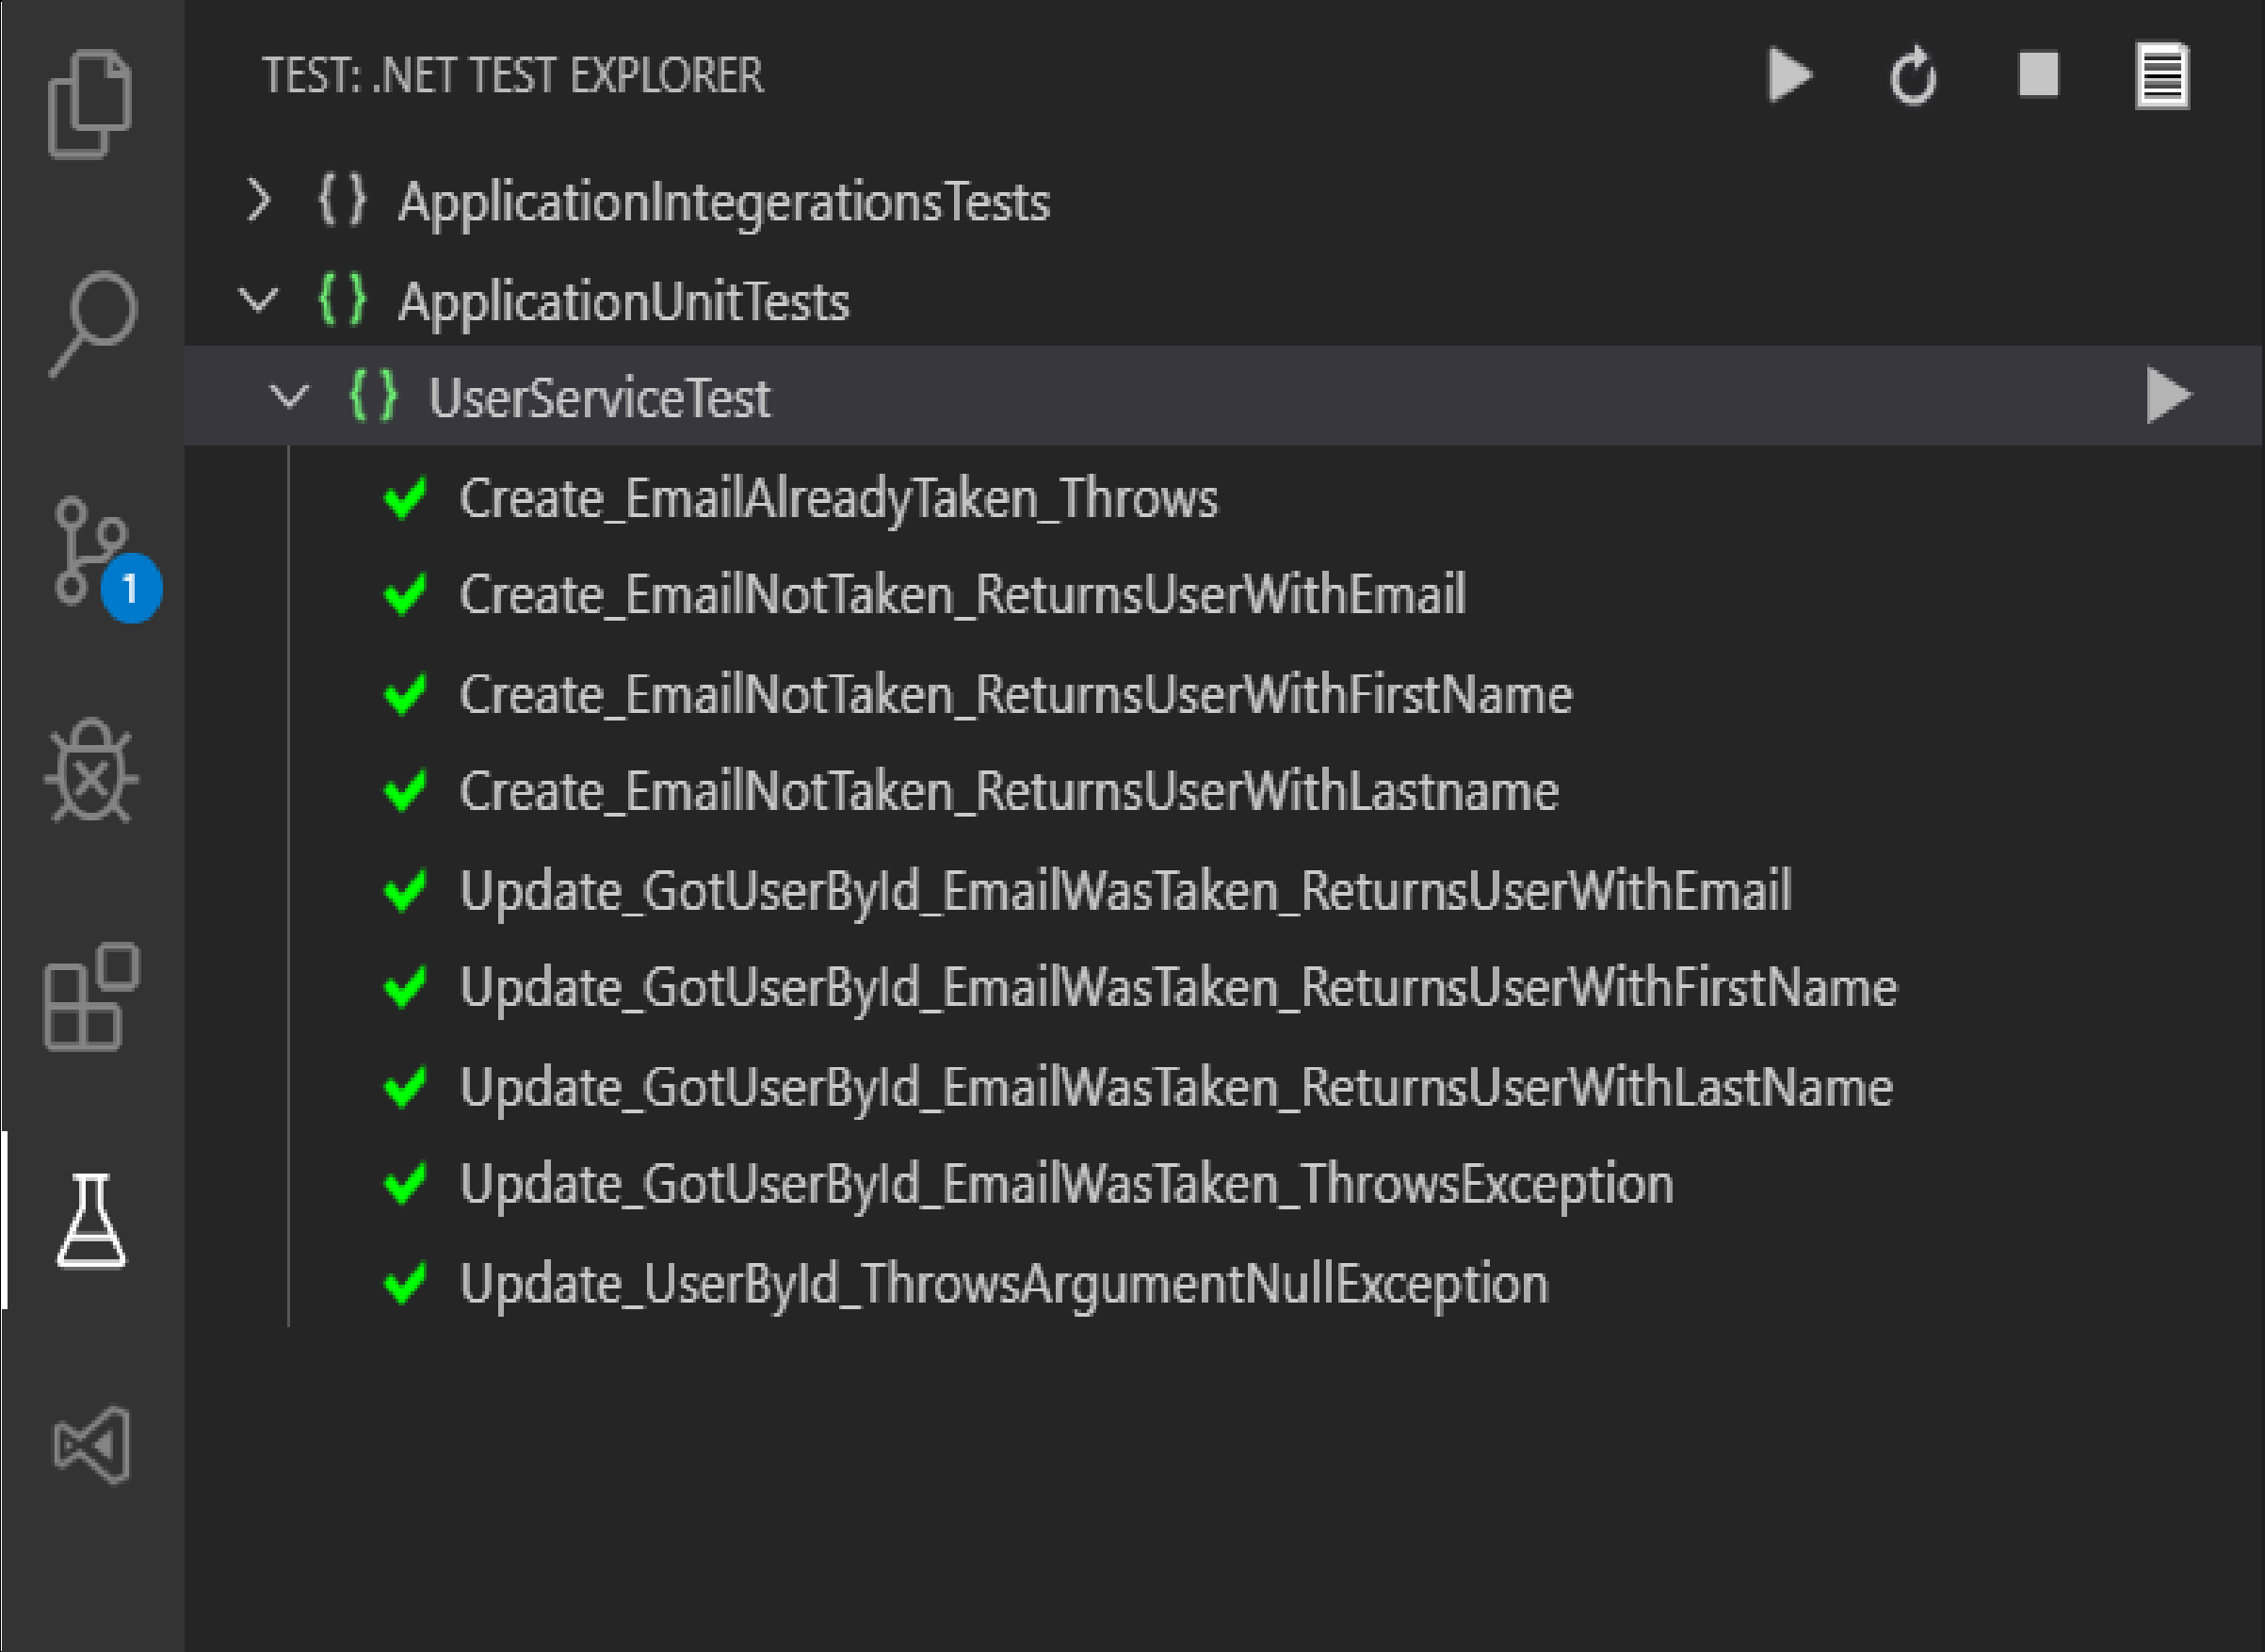
\includegraphics[width=0.6\textwidth]{Unit-Test-image/user-service-UnitTest.pdf}
\caption{Udsnit af unit-tests for user-service}
\label{fig:figure2}
\end{figure}

Ud fa ovenstående figur ses at der er udviklet 9 unit tests kun for user-servicen og sådan er det også for de resterende 13 services, hvor det består af omkring 8-15 test cases per service. 
